\documentclass[acmlarge]{acmart}
\settopmatter{printacmref=false} % Removes citation information below abstract
\renewcommand\footnotetextcopyrightpermission[1]{} % removes footnote with conference information in first column
\pagestyle{plain} % removes running headers

\usepackage{booktabs} % For formal tables


\usepackage[ruled]{algorithm2e} % For algorithms
\renewcommand{\algorithmcfname}{ALGORITHM}
\SetAlFnt{\small}
\SetAlCapFnt{\small}
\SetAlCapNameFnt{\small}
\SetAlCapHSkip{0pt}
\IncMargin{-\parindent}

% Metadata Information
%\acmJournal{PACMHCI}
%\acmVolume{9}
%\acmNumber{4}
%\acmArticle{39}
%\acmYear{2010}
%\acmMonth{3}
%\acmArticleSeq{11}

%\acmBadgeR[http://ctuning.org/ae/ppopp2016.html]{ae-logo}
%\acmBadgeL[http://ctuning.org/ae/ppopp2016.html]{ae-logo}


% Copyright
%\setcopyright{acmcopyright}
%\setcopyright{acmlicensed}
%\setcopyright{rightsretained}
%\setcopyright{usgov}
%\setcopyright{usgovmixed}
%\setcopyright{cagov}
%\setcopyright{cagovmixed}

%\ DOI
%\acmDOI{0000001.0000001}

% Paper history
%\received{February 2007}
%\received{March 2009}
%\received[accepted]{June 2009}


% Document starts
\begin{document}
% Title portion
\title{A Replication Study} 

\author{Bingquan Wang}
\affiliation{%
  \institution{University College London}
}

\begin{abstract}
Abstract
\end{abstract}

%
% End generated code
%


\keywords{}


\thanks{}


\maketitle

% The default list of authors is too long for headers}
%\renewcommand{\shortauthors}{B. Wang et al.}

\section{Introduction}
Software testing is essential to increase quality of programs. It validates whether a software system is working correctly according to specification by executing the piece of code against test cases. Earlier studies have already shown, for any meaningful program that finding all the faults and proving the program is faults-free is in practice undecidable. As complexity and input data range increase quickly over the years, ensuring the software system to achieve the desired level of quality is more and more difficult. There is always a trade-off between cost of improving testing and cost of leaving undetected faults in a program. It is necessary for developers to measure and predict test quality, given only the actual program and test cases run against it.

Test coverage is a measure of how much code of a program has been executed against a particular test suite. It is believed that higher the coverage, higher the chance to detect faults, because tests can never find faults which have never been executed. However, it is still an open question how strong test coverage criteria is related to effectiveness of detecting faults. There are different studies on this question, but an agreement has not been reached.

A common understanding of code coverage is that it is useful in finding non-executed code, but is less useful in finding non-tested data input. Figure is an example of why code coverage may not be a good measure. Let us suppose we need a piece of code to tell us if input is greater than zero. And the specification is that only when input is greater than zero return true, otherwise return false, as shown in Algorithm~\ref{algo:correctgreater} and Algorithm~\ref{algo:faultygreater}. By having a test suite containing test cases greater than zero and less than zero, both code achieves 100\% statement coverage. However, without testing zero specifically, faulty version of program can never be revealed.

\begin{algorithm}[h]	
	\KwData{Integer }
	\KwResult{return true when input is greater than 0 else return false }
	\eIf{A $>$ 0}{
		return true\;
	}
	{	return false\;
	}
	\caption{Determine if input is positive (correct)}
	\label{algo:correctgreater}
	\bigskip
\end{algorithm}

\begin{algorithm}[h]
	\KwData{Integer A}
	\KwResult{return true when input is greater than 0 else return false }
	\eIf{A $>=$ 0}{
		return ture\;
	}
	{
		return false\;
	}
	\caption{Determine if input is positive (faulty)}
	\label{algo:faultygreater}
	\bigskip
\end{algorithm}

The other technique of measuring test suite quality is mutation testing. Mutation testing tests whether test cases of the software system can detect small human seeded faults. The higher the mutation testing score, the better the test quality, which means it is able to find more human seeded faults. Mutation testing score is one of the most informative measure for quality of test suites as it is a direct measure of fault detection ability. However, there are also two problems with mutation testing. Firstly, human seeded faults are simulations of real faults which are not be the same as real software faults, so ability of finding human seeded faults may not be the same as ability of finding real faults. Another problem is that mutation is difficult to implement, and takes a long time to run. So mutation testing has not been recommended in industry. 

Both testing measures have their limitations. And mutation testing is not commonly accepted by industry. It is important for developers and researchers to know if they can still safely use code coverage as a good measure for testing quality. This project is a replication study of a recent paper "Code Coverage is Not Strongly Correlated With Test Suite Effectiveness".
\section{Related Work}
\label{sec:related}
Most previous work considered correlation of code coverage criteria and ability of finding number of faults. To determine the fault detection ability researches manually inserted known faults to programs, either previous fixed bugs or syntactic change, then measure the number of seeded faults a test suite can detect, which is essentially the same as mutation testing. Budd et al. proved mutation testing score is a stronger metric compare to other coverage criteria for test suite evaluation. Li et al, compared three code coverage criteria(edge pair, all use, prime path) with mutation testing, found that mutation testing is the best in detecting hand seeded faults in small programs. Despite the studies did not use large-scale SUTs, with the methodologies that minimise the bias, it is highly possible that mutation testing is better at evaluating test suites.

Wong et al.~\cite{wong1994effect} investigated correlation between fault detection effectiveness and block coverage and correlation between fault detection effectiveness and size. They found that there is a correlation between block coverage and fault detection effectiveness. Also correlation between block coverage and fault detection effectiveness is higher than correlation between size and fault detection effectiveness. For this study, they believe that increasing the number of test cases in a test suite without increasing its coverage does not increase fault detection effectiveness.

Hutchins et al.~\cite{hutchins1994experiments} 

Andrew et al.~\cite{andrews2006using} studied behaviour of random selecting test suites and test suites constructed by adding test cases to improve test coverage, that is for the latter test suite if a test case does not increase coverage for a test suite, it is discarded and a new test case is selected. They found that for test suites with the same size, test suites consider coverage results better test effectiveness. Indirectly, it is saying there is a correlation between test effectiveness and coverage.

A study by Namin et al.~\cite{namin2009influence} claimed that both coverage and size have effect on test suite effectiveness. They found a non-linear relationship between test suite size, coverage and test suite effectiveness. They introduced a maths model (log(size) + coverage) which they believed can be used to predict the test suite effectiveness.

Cai et al.~\cite{cai2005effect} investigated relationship between test effectiveness and coverage metrics under different test profile: whole test set, functional test, random test, normal test, exceptional test. They found that for exceptional test, there is a significant correlation between test effectiveness and code coverage. There is no correlation for normal test. There is moderate correlation for functional and random test.


Gligoric et al.~\cite{gligoric2013comparing} measured both Kendall and Pearson to examine correlations to mutation kill for a set of criteria, Their work considers 15 Java programs and 11 C programs, selected not randomly but primarily from container classes used in previous studies and the classic Siemens subjects. Their larger projects (JodaTime, JFreeChart, SQLLite, YAFFS2) were chosen opportunistically. The study suggested that the correlation between coverage and effectiveness in real systems
is largely due to the correlation between coverage and size; it also suggested that results from automatically generated and manually generated suites do not generalize to each other.

Gopinath et al.~\cite{gopinath2014code} measured mutation score and coverage for more than 200 programs for their master suite and automatically generated test suites. They found there is correlation between coverage criteria and fault detection effectiveness for master suites and automatically generated suites. The correlation for master suite is stronger compare to automatically generated suites. They also claim that adding automatically generated suites to master suite does not necessarily increase test effectiveness. So size of test suite is not strongly correlated with effectiveness. (This is Alex work, the other paper we wanted to replicate)

This replication study is about a resent work from Inozemtseva et al.~\cite{inozemtseva2014coverage}. They studied correlation between different coverage and test effectiveness.

Unlike ealier studies which most of them used mutation testing score directly as effectiveness of fault detection. Inozemtseva et al.~\cite{inozemtseva2014coverage} defined two effectiveness measures, \textit{raw effectiveness measurement} and \textit{normalised effectiveness measurement}. "The raw kill score is the number of mutants a test suite detected divided by the total number of
non-equivalent mutants that were generated for the subject program under test."~\cite{inozemtseva2014coverage}. "The normalized effectiveness measurement is the number of mutants a test suite detected divided by the number of non-equivalent mutants it covers."~\cite{inozemtseva2014coverage}. A test suite cover the mutant means test cases in the test suite execute the mutated line of code. Or the mutant can be detected by the test suite. 

The reason to introduce this normalised effectiveness is that when size of test suite is controlled, there are limited lines of code and mutants it covers. Authors are more interested in effectiveness relative to the test suite itself. For example, test suite A kills 10 mutants and test suite B kills 100 mutants, for raw effectiveness suite B is certainly higher. If suite A only has 12 covered non-equivalent mutants and suite B has 200, suite A will have a higher normalised effectiveness than suite B. The definition of normalised effectiveness captures the idea that an effective suite is very good at finding faults with in the code that it runs.

The result of Inozemtseva et al.'s work is that when test suite size is not controlled, there is moderate to high correlation between all code coverage criteria and effectiveness; when test suite size is controlled, there is low to moderate correlation between all coverage types and effectiveness. Also saying size is a correlated with effectiveness.

As above studies show, most studies claim that there is some relationship between coverage, size and test effectiveness. But they do not agree to each other about how strong the relationship is.
\section{Concept}
\subsection{Testing Terminology}
Terminologies used for testing in general and for this paper are defined as follows:
\begin{itemize}
	\item Test case/methods: a independent unit test. It isolates a fragment of code (normally a functional method) and validates its correctness. Ideally, unit test should not go outside its own method boundary. When methods interact with each other, it is more difficult to identify which component is the cause of failure. Test cases are sometimes also called test methods.
	\item Test suite: a collection of test cases which are used to validate a set of behaviour.
	\item Master test suite: A test suite contain all test cases written by developer. In this paper, all test suites evaluated are strict subsets of the master test suite.
\end{itemize}
\subsection{Mutation Testing}
Mutation testing is a technique which tests if test suite can detect human seeded faults. Faulty programs are created by changing original program syntax which is called a \textbf{mutant}, each mutant contains a different syntactic change. Every mutant is executed against test suites, if the result is different to the original program, then the mutant is \textbf{killed}, otherwise the mutant has \textbf{survived}.

For a surviving mutant, there are two possible reasons for it to happen. Either the test suite does not contain test cases cover the fault, or the mutant is syntactically different but semantically the same. Those mutants semantically the same can never be killed, which are called \textbf{equivalent mutants}. For example, Algorithm~\ref{algo:A>B} is identical to algorithm~\ref{algo:A>=B} in terms of functionality. A particular mutant changing algorithm~\ref{algo:A>B} to algorithm~\ref{algo:A>=B} can never be detected. Mutation score by formal definition is the ratio of number of killed mutants over the number of non-equivalent mutants~\cite{jia2011analysis}. 

\begin{algorithm}[H]
	\label{algo:A>B}
	\KwData{Integer A and Interger B}
	\KwResult{Return the number with highest value }
	\eIf{A $>$ B}{
		return A\;
	}
	{return B\;
	}
	\caption{Return the number with highest value}
\end{algorithm}

\bigskip

\begin{algorithm}[H]
	\label{algo:A>=B}
	\KwData{Integer A and Interger B}
	\KwResult{Return the number with highest value }
	\eIf{A $>=$ B}{
		return A\;
	}
	{
		return B\;
	}
	\caption{Return the number with highest value}
\end{algorithm}

Determine if a survived mutant is equivalent is undecidable for computers as shown in the previous study~\cite{budd1982two}. Currently, a very common practice in research is to assume the test suite is adequate and treat all surviving mutants as equivalent mutants~\cite{jia2011analysis}. This is a overestimation of equivalent mutants but allows researchers to work on large programs.

\subsection{Coverage Criteria}
There are three coverage criteria used in the project: statement, decision and modified condition coverage.

Statement coverage is the percentage of how many lines of statements have been executed for a particular test suite. 

Decision coverage

Modified condition coverage(MCC)
\subsection{Effectiveness}
As mentioned in Section~\ref{sec:related}, there are two effectiveness introduced in this paper: raw effectiveness measurement and normalised effectiveness measurement. Author did not give mathematical expression for two effectiveness.

Raw effectiveness is the number of killed mutants of a test suite divided by the number of killed mutants of master test suite. For a test suite t, master suite T and program P, raw effectiveness should be:
\[\textit{rawEffectiveness} = \frac{\#\textit{killedMutants(t,P)}}{\#\textit{killedMutants(T,P)}}\]

For a test suite normalised effectiveness and is calculated by killed mutants of this suite over covered non-equivalent mutants of the same suite. Directly from authors' definiation we have the expression, for a test suite t and program P:
\[\textit{normalisedEffectiveness} = \frac{\#\textit{killedMutants(t,P)}}{\#\textit{coveredNon-equivalentMutants(t,P)}}\]

Covered non-equivalent mutants need further decomposition. A mutant can have three status for a particular test suite: covered and killed by test cases in this test suite, covered but not killed by this test suite but killed by test cases outside this test suite and surviving or equivalent. Covered non-equivalent mutants are total mutants covered taking away surviving mutants. So the final equation of normalised effectiveness for a test suite t and program P is:
\[\textit{normalisedEffectiveness} = \frac{\#\textit{killedMutants(t,P)}}{\#\textit{totalCoveredMutants(t,P)} - \#\textit{equivalentMutants(t,P)}}\]
\subsection{Correlation Measurement}
\section{Methodology}
\subsection{Procedure}
The procedure used in this research is as follows:
\begin{enumerate}
	\item Use a mutation testing tool(PIT) to produce faulty program and run mutants against master test suite. Get mutant status for every test case.
	\item Generate a large number of test suites by randomly selecting tests cases from master test suite, until the test suite reaches its pre-defined size.
	\item For each test suite:
	\begin{itemize}
		\item Measure coverage criteria (CodeCover) for different test suites.
		\item Determine effectiveness of different test suites using mutation information and coverage criteria.
	\end{itemize}
	\item Analyse correlation between different coverage criteria and effectiveness.
\end{enumerate}

\subsection{Subjects under test}
The original paper used five following subject programs: 
\begin{enumerate}
	\item Apache POI~\cite{apachepoi}: a Java API for Microsoft Documents
	\item Closure~\cite{closure}: a tool for making JavaScript download and run faster.
	\item HSQLDB~\cite{hsqldb}: a Java SQL relational database.
	\item JfreeChart~\cite{jfreechart}: a Java chart library for users to display professional quality charts.
	\item Joda Time~\cite{jodatime}: A replacement for Java time and date class
\end{enumerate}

These five subjects are selected on purpose using the following criteria:
\begin{enumerate}
	\item The program needs to be large enough to have more than 100,000 SLOC;
	\item It needs to be an actively developed Java program;
	\item It contains at least 1000 test cases;
	\item The project needs to use Ant as its build system;
	\item The project uses JUnit as a test harness.
\end{enumerate}

However no versions or git hashes of subject programs were given in the original paper or in its artefact page. As the original paper was published in 2014, various number of test subjects versions between 2012 to 2014 were examined with different PIT versions, but there was no result that was close enough to what was reported in the original paper. Figure~\ref{fig:jodamutant} and figure~\ref{fig:jodakilled} are examples of different versions of Joda Time running against PIT version 1.0.0. We contacted authors of the original paper, and acquired their project repository.


\begin{figure}
	\centering
	\begin{minipage}{0.4\textwidth}
		\centering
		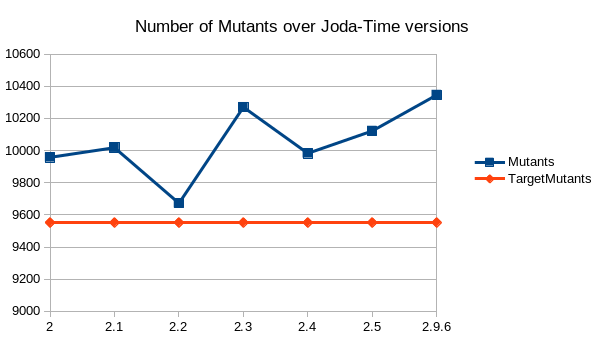
\includegraphics[width=\textwidth]{Figure/joda_mutant.png}
		\caption{Joda Time total mutants}
		\label{fig:jodamutant}
	\end{minipage} %
	\begin{minipage}{0.4\textwidth}
		\centering
		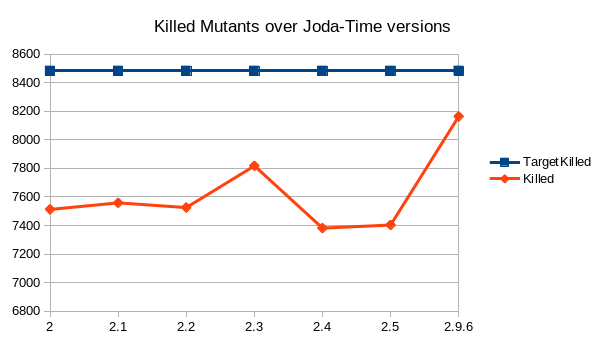
\includegraphics[width=\textwidth]{Figure/joda_kill.png}
		\caption{Joda Time killed mutants}
		\label{fig:jodakilled}
	\end{minipage}
\end{figure}

There are some environment settings need to be adjusted locally. Mutation testing tool PIT used for this project requires green test suite, which means all tests must pass. During my replication, some projects provided by the author could not compile or did not pass all tests. The first Java compiler used in the replication was Java 8, but non of the projects passed all tests. HSQLDB, JfreeChart, Joda Time worked with no errors using Java 7. According to ant build system, recommanded Java compiler for Closure was Java 6, but non of the compiler version complied it successfully. For Apache POI, Java 6 and 7 compilation was successful but resulted failing tests.

There was no command to exclude failing tests in author's repository, and the report log suggests the Apache POI and Closure were working correctly. I downloaded source code from GitHub according to author's repository. Table~\ref{tab:sut} is a summary of projects and compiler version. Java 7 was selected as final replication compiler.


\begin{table}
	\caption{Java Compiler Setting}
	\label{tab:sut}
	\begin{minipage}{\columnwidth}
		\begin{center}
			\begin{tabular}{|l|l|c|c|c|c|c|c|}
				\hline
				&&\multicolumn{2}{|c|}{Java 6}&\multicolumn{2}{|c|}{Java 7}&\multicolumn{2}{|c|}{Java 8}\\
				\hline
				Project & Version & Compile & Test & Compile & Test & Compile & Test \\
				\hline
				Apache POI & 3.9(author) & Success & Fail & Success & Fail & Success & Fail \\
				& 3.9(GitHub) & Success & Success& Success& Success & Success& Fail \\
				\hline
				Closure& 20130227(author) & Fail & Fail & Fail & Fail & Fail & Fail \\
				&20130227(GitHub) & Success & Success & Success & Success & Success & Fail \\
				\hline
				HSQLDB & 2.2.8 & Success & Success & Success & Success & Success & Fail \\
				\hline
				JfreeChart & 1.0.8 & Success & Success & Success & Success & Success & Fail \\
				\hline
				Joda Time & 2.0 & Success & Success & Success & Success & Success & Fail \\
				\hline
			\end{tabular}
		\end{center}
		\bigskip
	\end{minipage}
\end{table}

The final environment settings used in this replication study are:
\begin{itemize}
	\item Operating System: Ubuntu 14.04.5 LTS;
	\item Java Compiler: 1.7.0\_u131;
	\item ant build system: 1.9.3;
	\item JUnit: 3.8 for compiling projects, 4.10 for running PIT;
	
Other systems should work, as long as using Java compiler 7, ant version greater than 1.8; and having JUnit 3 and JUnit 4  at the same time.
\end{itemize}


\subsection{Mutation Testing}
Mutation testing of the program was conducted using an automated mutilation testing tool PIT. 
\subsection{Test suite generation}
\subsection{Coverage Measurement}
\subsection{Measuring Effectiveness}
\input{repDetail.tex}
\section{Results}
\subsection{PIT results}
\label{subsec:resultPIT}
At the beginning of our replication, with authors' SUT repositories and her suggested modified version of PIT, we were not able to reproduce results that were close enough to the original paper. We contacted author for help, she helped us to understand her log file and how she got the results.

As mentioned in section~\ref{subsec:mutationTesting}, for authors' modified PIT, there are information for every mutant and its corresponding test cases. For the number of surviving mutants, she counted the number of mutants logged as survived in her modified log. The number of detected mutants was calculated by subtracting number of surviving mutants from number of total generated mutants.

However, PIT is more complicated than just have killed and surviving mutants as shown in section~\ref{subsec:mutationTesting}. Under normal circumstances, mutants can also have outcomes of not covered and time out. Whether not covered mutants are killed or surviving can not be detected by current test suite, so they are not reported as killed or surviving mutants. Time out mutants are considered as killed as they cause a infinite loop and force PIT to move to next mutant. Therefore the way she generate killed mutants was wrong, she did not consider mutants with outcome of not covered. Table~\ref{tab:pit} includes information extracted from her repository and paper without running PIT. 

For Apache POI, number of equivalent mutants reported in the paper is the same as adding surviving mutants and no covered mutants in PIT default report. Also number of killed mutants match with PIT default report. However for the other four projects, number of surviving mutants in the paper match with modified PIT log, and the number of killed mutants are calculated using total number of generated mutants subtract number of surviving mutants. From this we can tell for all five mutants, the numbers reported in the paper were wrong for two reasons. Firstly, not covered mutants were not considered. Secondly, the way she calculated the number of killed mutants was inconsistent.

Furthermore, looking at PIT default report and modified report, number of survived mutants do not match. For Apache PIT, Closure, JfreeChart and Joda Time, the difference is very small and can be accepted. But for HSQLDB, the difference is too significant to ignore. We investigated the cause, during the running of PIT, there were lots of standard error output. For normal process, if there are errors, PIT aborts and reports them. However, for HSQLDB, PIT run successfully along with reporting errors. PIT is a very complex system, it was not possible for us to resolve the problem and modify it to give correct results in the given time. Thus, we decided to discard usage of HSQLDB.

\begin{table}[h]
	\caption{PIT Report}
	\label{tab:pit}
	\begin{minipage}{\columnwidth}
		\begin{center}
			\begin{tabular}{|c|c|c|c|c|c|c|}
				\hline
				&Property & Apache POI & Closure & HSQLDB& JFreeChart & Joda Time \\
				\hline
				Original Paper & Generated Mutant & 27565 & 30779& 50302 & 29699 & 9552\\
				& Detected mutant & 17935 & 27325 & 50125 &23585 & 8483\\
				& Equivalent mutant & 9630 & 3454 & 177 &6114 & 1069\\
				\hline
				PIT default log & Generated Mutant & 27565 & 30779& 50302 & 29699 & 9552\\
				& Killed mutant & 17935 & 23178 & 8150 &9808 & 7503\\
				& Survived & 3458 & 3447 & 5376 &6106 & 1066\\
				& Not covered & 6172 & 4154 & 36775 & 13785 & 983\\
				& Survived + no covered & 9630 & 7601 & 42152 & 19891 & 2049\\
				\hline
				Modified log & Surviving mutant & 3469& 3454& 177 & 6125& 1069\\
				\hline
			\end{tabular}
		\end{center}
		\bigskip
	\end{minipage}
\end{table}

Table~\ref{tab:pitrep} is PIT mutation testing replication result. For Apache POI and Closure, we fetched repository from GitHub as authors' could not compile and test straight away. For JFreeChart, and Joda time, we used repository as author provided. We used authors' modified PIT, as it provides essential mutant outcome for correlation analysis. For these four projects, we have got similar PIT results to original paper. The difference can be caused by randomness of PIT automation and different Java compiler version. The replication PIT results are used for further analysis in this study.

\begin{table}[h]
	\caption{Replication PIT Report}
	\label{tab:pitrep}
	\begin{minipage}{\columnwidth}
		\begin{center}
			\begin{tabular}{|c|c|c|c|c|c|}
				\hline
				&Property & Apache POI & Closure & JFreeChart & Joda Time \\
				\hline
				PIT default log & Generated Mutant & 27565 & 30779 & 29699 & 9552\\
				& Killed mutant & 17923 & 22841  &9868 & 7486\\
				& Survived & 3466 & 3515 &6109 & 1074\\
				& Not covered & 6176 & 4423 & 13722 & 992\\
				\hline
				Modified log & Surviving mutant & 3472 & 3518 & 6122& 1076\\
				\hline
			\end{tabular}
		\end{center}
		\bigskip
	\end{minipage}
\end{table}

\subsection{Is Coverage Correlated With Effectiveness When Size Is Ignored?}
When we analysis authors' data used for raw effectiveness, we found that the number of total killed mutants used in the calculation was wrong. Recall section~\ref{subsec:resultPIT} that row of detect mutant in table~\ref{tab:pit} also counts not covered mutant for three project: Closure, JFreeChart and Joda Time. These numbers were used as total killed mutants when calculating raw effectiveness. Thus the actual raw effectiveness for those three projects is:
For random subtest t, master suite T and program P
\[\textit{rawEffectiveness} = \frac{\#\textit{killedMutants(t,P)}}{\#\textit{killedMutants(T,P)} + \#\textit{notCoveredMutants(T,P)}}\]

However this misuse of killed mutants did not affect overall correlation result. Adding total not covered mutants does not effect the ranking of raw effectiveness. Since correlation only interests in ranking of value,  In addition we validated the results of raw effectiveness by changing total number of killed mutants to what was reported in PIT default log and got identical results. So the raw effectiveness correlation of original is still valid despite the mistake of detected mutants.


Our first interest is whether coverage is correlated with fault detection effectiveness when size is ignored. Table~\ref{tab:rawnosize} and table~\ref{tab:normalnosize} show the Kendall $\tau$ correlation coefficients for raw effectiveness and normalised effectiveness discussed in section~\ref{subsec:effectiveness}. All 4 projects showed high correlation between raw effectiveness and coverage criteria. When normalisation applied, the correlation decreased for every subject. JFreeChart drooped the most, from very high correlation to moderate while other projects still maintain high. So we can conclude that there is moderate to high correlation between coverage criteria and fault detection effectiveness when size is ignored. In other words, when size of test suite is ignored, the higher the coverage the more faults a test suite can detect fault. 

\begin{table}[h]
	\caption{Kendall correlation between raw effectiveness and coverage criteria when size is ignored}
	\label{tab:rawnosize}
	\begin{minipage}{0.7\columnwidth}
		\begin{center}
			\begin{tabular}{cccc|ccc}
				\hline
				& \multicolumn{3}{c}{Original} & \multicolumn{3}{c}{Replication} \\
				\hline
				Project & Statement & Decision & MCC & Statement & Decision & MCC  \\
				\hline
				Apache POI & 0.94 & 0.94 & 0.94 & 0.92 & 0.94 & 0.94 \\
				JFreeChart & 0.91 & 0.95 & 0.92 & 0.90 & 0.92 & 0.90\\
				Joda Time & 0.85 & 0.85 & 0.85 & 0.94 & 0.94 & 0.93 \\
				\hline
			\end{tabular}
		\end{center}
		\bigskip
		\emph{Note:} All entries are significant at 99\% level
	\end{minipage}
\end{table}

\begin{table}[h]
	\caption{Kendall correlation between normalised effectiveness and coverage criteria when size is ignored}
	\label{tab:normalnosize}
	\begin{minipage}{0.7\columnwidth}
		\begin{center}
			\begin{tabular}{cccc|ccc}
				\toprule
				& \multicolumn{3}{c}{Original} & \multicolumn{3}{c}{Replication} \\
				\hline
				Project & Statement & Decision & MCC & Statement & Decision & MCC  \\
				\hline
				Apache POI & 0.75 & 0.76 & 0.77 & 0.77& 0.77 & 0.81 \\
				JFreeChart &0.50 & 0.53 & 0.53 & 0.55 & 0.57 & 0.57 \\
				Joda Time & 0.80 & 0.80 & 0.80 & 0.84 & 0.84 & 0.84 \\
				\hline
			\end{tabular}
		\end{center}
		\bigskip
		\emph{Note:} All entries are significant at 99\% level
	\end{minipage}
\end{table}



\subsection{Is Coverage Correlated With Effectiveness When Size Is Controlled?}
We computed the Kendall τ correlation coefficient between effectiveness and coverage for each project, each suite size, each coverage type, and both effectiveness measures.

In general, when test suite size was controlled, raw effectiveness measurements had moderate correlations with coverage and normalized effectiveness measurements had low to moderate correlations.

For Joda Time, our replication result was very different to original paper as shown in Table~\ref{tab:jodaraw} and Table~\ref{tab:jodanorm}. For both raw and normalised effectiveness, original paper had near zero correlations for all type of coverage and any size. However, according to our replication, there is moderate correlation between raw effectiveness and all three coverage, and there is low correlation between normalised effectiveness and coverage.


\begin{table}[h]
	\caption{Apache POI Raw}
	\label{tab:poiraw}
	\begin{minipage}{0.7\columnwidth}
		\begin{center}
			\begin{tabular}{cccc|ccc}
				\toprule
				& \multicolumn{3}{c}{Original} & \multicolumn{3}{c}{Replication} \\
				\hline
				Size & Statement & Decision & MCC & Statement & Decision & MCC  \\
				\hline
				3   & 0.85 & 0.84 & 0.85 & 0.80 & 0.81 & 0.80\\
				10  & 0.75 & 0.73 & 0.77 & 0.75 & 0.77 & 0.77\\
				30  & 0.61 & 0.67 & 0.67 & 0.56  & 0.58  & 0.58 \\
				100 & 0.51 & 0.48 & 0.46 & 0.55  & 0.52  & 0.55 \\
				300 & 0.67 & 0.64 & 0.63 & 0.60  & 0.63  & 0.60 \\
				1000 & 0.77 & 0.63 & 0.69 & 0.79  & 0.72 & 0.64 \\
				\bottomrule
			\end{tabular}
		\end{center}
		\bigskip
		\emph{Note:} All entries are significant at 99\% level
	\end{minipage}
\end{table}

\begin{table}[h]
	\caption{Apache POI Normalised}
	\label{tab:poinorm}
	\begin{minipage}{0.7\columnwidth}
		\begin{center}
			\begin{tabular}{cccc|ccc}
				\toprule
				& \multicolumn{3}{c}{Original} & \multicolumn{3}{c}{Replication} \\
				\hline
				Size & Statement & Decision & MCC & Statement & Decision & MCC  \\
				\hline
				3   & -0.17 & -0.13 & -0.07 & -0.09\textborn & -0.08\textborn & -0.01\textborn \\
				10  & 0.14 & 0.16 & 0.22 & 0.18 & 0.20 & 0.20\\
				30  & 0.18 & 0.27 & 0.28 & 0.22 & 0.21  & 0.21 \\
				100 & 0.15 & 0.21 & 0.21 & 0.27  & 0.30  & 0.32 \\
				300 & 0.41 & 0.40 & 0.42 & 0.52  & 0.45  & 0.46 \\
				1000 & 0.49 & 0.46 & 0.49 & 0.49  & 0.48 & 0.48 \\
				\bottomrule
			\end{tabular}
		\end{center}
		\bigskip
		\emph{Note:} All entries are significant at 99\% level
	\end{minipage}
\end{table}

\begin{table}[h]
	\caption{Apache POI Raw}
	\label{tab:closureraw}
	\begin{minipage}{0.7\columnwidth}
		\begin{center}
			\begin{tabular}{cccc|ccc}
				\toprule
				& \multicolumn{3}{c}{Original} & \multicolumn{3}{c}{Replication} \\
				\hline
				Size & Statement & Decision & MCC & Statement & Decision & MCC  \\
				\hline
				3   & 0.79 & 0.80 & 0.80 &  &  & \\
				10  & 0.71 & 0.72 & 0.69 &  &  & \\
				30  & 0.69 & 0.73 & 0.70 &   &   &  \\
				100 & 0.70 & 0.66 & 0.57 &   &   &  \\
				300 & 0.65 & 0.62 & 0.56 &   &   &  \\
				1000 & 0.52 & 0.52 & 0.46 &  &  &  \\
				\bottomrule
			\end{tabular}
		\end{center}
		\bigskip
		\emph{Note:} All entries are significant at 99\% level
	\end{minipage}
\end{table}

\begin{table}[h]
	\caption{Closure Normalised}
	\label{tab:closurenorm}
	\begin{minipage}{0.7\columnwidth}
		\begin{center}
			\begin{tabular}{cccc|ccc}
				\toprule
				& \multicolumn{3}{c}{Original} & \multicolumn{3}{c}{Replication} \\
				\hline
				Size & Statement & Decision & MCC & Statement & Decision & MCC  \\
				\hline
				3   & 0.12 & 0.14 & 0.18 &  &  &  \\
				10  & -0.14 & -0.13 & -0.04\textborn & &&\\
				30  & -0.27 & -0.22 & -0.16 & && \\
				100 & -0.04\textborn & -0.03\textborn & -0.01\textborn & && \\
				300 & 0.12 & 0.12 & 0.15 & && \\
				1000 & 0.12 & 0.10 & 0.13 & && \\
				3000 & 0.13 & 0.17 & 0.19 &&&\\
				\bottomrule
			\end{tabular}
		\end{center}
		\bigskip
		\emph{Note:} All entries are significant at 99\% level
	\end{minipage}
\end{table}
 
\begin{table}[h]
	\caption{Closure Raw}
	\label{tab:jfreeraw}
	\begin{minipage}{0.7\columnwidth}
		\begin{center}
			\begin{tabular}{cccc|ccc}
				\toprule
				& \multicolumn{3}{c}{Original} & \multicolumn{3}{c}{Replication} \\
				\hline
				Size & Statement & Decision & MCC & Statement & Decision & MCC  \\
				\hline
				3   & 0.70 & 0.84 & 0.56 & 0.73 & 0.85 & 0.57\\
				10  & 0.66 & 0.83 & 0.68 & 0.59 & 0.68 & 0.56\\
				30  & 0.65 & 0.78 & 0.69 & 0.40  & 0.40  & 0.37 \\
				100 & 0.53 & 0.68 & 0.57 & 0.33  & 0.39  & 0.38 \\
				300 & 0.46 & 0.64 & 0.56 & 0.40  & 0.54  & 0.51 \\
				1000 & 0.46 & 0.62 & 0.60 & 0.38  & 0.60 & 0.59 \\
				\bottomrule
			\end{tabular}
		\end{center}
		\bigskip
		\emph{Note:} All entries are significant at 99\% level
	\end{minipage}
\end{table}

\begin{table}[h]
	\caption{JfreeChart Normalised}
	\label{tab:jfreenorm}
	\begin{minipage}{0.7\columnwidth}
		\begin{center}
			\begin{tabular}{cccc|ccc}
				\toprule
				& \multicolumn{3}{c}{Original} & \multicolumn{3}{c}{Replication} \\
				\hline
				Size & Statement & Decision & MCC & Statement & Decision & MCC  \\
				\hline
				3   & -0.25 & -0.08 & -0.20 & -0.20 & -0.06\textborn & -0.18\\
				10  & -0.42 & -0.26 & -0.33 & -0.32 & -0.21 & -0.26\\
				30  & -0.28 & -0.17 & -0.19 & -0.02\textborn  & 0.03\textborn  & 0.05\textborn \\
				100 & -0.09 & -0.01\textborn & 0.03\textborn & 0.00\textborn  & 0.08  & 0.14 \\
				300 & 0.03\textborn & 0.11 & 0.20 & 0.01\textborn  & 0.10  & 0.21 \\
				1000 & 0.06 & 0.13 & 0.20 &0.06\textborn  & 0.13 & 0.18 \\
				\bottomrule
			\end{tabular}
		\end{center}
		\bigskip
		\emph{Note:} Entry marked with \textborn~is not significant at 99\% level
	\end{minipage}
\end{table}

\begin{table}[h]
	\caption{Joda Time Raw}
	\label{tab:jodaraw}
	\begin{minipage}{0.7\columnwidth}
		\begin{center}
			\begin{tabular}{cccc|ccc}
				\toprule
				& \multicolumn{3}{c}{Original} & \multicolumn{3}{c}{Replication} \\
				\hline
				Size & Statement & Decision & MCC & Statement & Decision & MCC  \\
				\hline
				3   & -0.04\textborn & -0.03\textborn & -0.05\textborn & 0.48 & 0.56 & 0.50\\
				10  & 0.01\textborn & 0.00\textborn & 0.00\textborn & 0.52 & 0.60 & 0.54\\
				30  & 0.00\textborn & 0.00\textborn & 0.00\textborn & 0.56  & 0.61  & 0.56 \\
				100 & 0.00\textborn & 0.01\textborn & 0.04\textborn & 0.55  & 0.60  & 0.55 \\
				300 & 0.03\textborn & 0.04\textborn & 0.04\textborn & 0.60  & 0.63  & 0.59 \\
				1000 & 0.00\textborn & 0.01\textborn & 0.00\textborn & 0.69  & 0.72 & 0.64 \\
				3000 & -0.01\textborn & 0.00\textborn & 0.00\textborn & 0.59 & 0.69 & 0.53 \\
				\bottomrule
			\end{tabular}
		\end{center}
		\bigskip
		\emph{Note:} Entry marked with \textborn~is not significant at 99\% level
	\end{minipage}
\end{table}

\begin{table}[h]
	\caption{Joda Time Normalised}
	\label{tab:jodanorm}
	\begin{minipage}{0.7\columnwidth}
		\begin{center}
			\begin{tabular}{cccc|ccc}
				\toprule
				& \multicolumn{3}{c}{Original} & \multicolumn{3}{c}{Replication} \\
				\hline
				Size & Statement & Decision & MCC & Statement & Decision & MCC  \\
				\hline
				3   & -0.00\textborn & -0.00\textborn & -0.00\textborn & -0.00\textborn & -0.00\textborn & -0.01\textborn \\
				10  & -0.02\textborn & -0.01\textborn & -0.01\textborn & 0.19 & 0.21 & 0.20\\
				30  & -0.00\textborn & -0.00\textborn & -0.01\textborn & 0.15 & 0.17  & 0.21 \\
				100 & -0.00\textborn & -0.01\textborn & 0.02\textborn & 0.27  & 0.30  & 0.32 \\
				300 & 0.03\textborn & 0.04\textborn & 0.04\textborn & 0.33\textborn  & 0.35  & 0.36 \\
				1000 & 0.00\textborn & 0.00\textborn & 0.00\textborn & 0.39  & 0.42 & 0.43 \\
				3000 & -0.04\textborn & -0.03\textborn & - 0.02\textborn &0.10 & 0.15 & 0.18\\
				\bottomrule
			\end{tabular}
		\end{center}
		\bigskip
		\emph{Note:} Entry marked with \textborn~is not significant at 99\% level
	\end{minipage}
\end{table}


\section{Conclusion}
\bibliographystyle{ACM-Reference-Format}
\bibliography{sample-bibliography}


\end{document}
